\documentclass[11pt,a4paper,italian]{article}
\usepackage{times}
\usepackage[T1]{fontenc}
\usepackage[latin1]{inputenc}
\usepackage{graphicx}


\makeatletter
\usepackage{babel}
\makeatother
\begin{document}

\newcommand{\fx}[0]{\texttt}

\title{Note sulla realizzazione del sistema di caching \\
per il Proxy RTSP di Real Networks}


\author{Merli Matteo\\
\fx{\footnotesize matteo.merli@studenti.unipr.it}}

\maketitle

\section{Stato attuale}

Al momento � stata implementata solamente un piccola parte delle
funzionalit� di caching del proxy. In particolare l'unica funzionalit�
presente � un primo abbozzo del sistema di salvataggio su disco dei
pacchetti ricevuti dal server.

Quando viene intercettata la richiesta \fx{SETUP} da parte
del client, si procede alla verifica della presenza in cache della
risorsa richiesta. Se questa viene trovata (\fx{CACHE HIT}), per
adesso non succede nulla in quanto non � presente il sistema di
trasmissione dei pacchetti presenti in cache. Se invece la risorsa non
era in cache (\fx{CACHE MISS}) viene attivato il meccanismo di
salvataggio dei pacchetti su disco.

I pacchetti vengono intercettati durante l'invio al client e vengono
scritti su disco tramite la classe \fx{CacheSegment}.
Ci� funziona testando il tutto con lo streaming di un file Mp3, a
parte il fatto che in realt� viene salvato su disco un numero di
pacchetti leggermente superiore a quello dei pacchetti effettivamente
ricevuti dal client.

Un test con RealPlayer One (utilizzando \fx{RDT} come protocollo di
trasporto) ha mostrato che il client riceveva 3425 pacchetti, mentre il
server ne registrava su disco 3430. Questo pu� essere dovuto al fatto
che venga salvato anche qualche pacchetto contenente ``strani''
segnali di controllo. Provando con openRTSP (che utilizza \fx{RTP}) i
pacchetti intercettati dal proxy sono stati 3448. 

Eseguendo prove con file audio/video, si presenta invece il problema
di salvare le due stream in 2 file separati. Questa operazione viene
complicata dal diverso modo di gestire lo streaming tra RTP e il
protocollo RDT di RealNetworks.

Quando lo streaming avviene con RTP/RTCP, il client ed il server
utilizzano entrambi 2 coppie di porte UDP per la comunicazione. Una
coppia di porte viene dedicata alla stream audio, mentre l'altra
coppia alla stream video. Questa configurazione non presenta
particolari difficolt�, possono venire creati 2 \fx{CacheItem} ed
ad ognuno verr� associato ad un canale di comunicazione.

Quando la comunicazione avviene invece con RDT, client e server
utilizzano una sola porta per tutti i dati, pacchetti audio e video e
segnali di controllo. Risulta quindi difficile separare le due
stream e probabilmente non ha nemmeno senso separarle, visto che il
client riesce comunque a distinguere quali sono i pacchetti della
stream audio e quali quelli video. Il problema in questo caso � che
viene comunque creato due \fx{CacheSegment}, ma uno di essi non viene
utilizzato e rimane vuoto. Questa situazione potrebbe portare dei
problemi successivamente duranta la fase di invio dei pacchetti
cachati da parte del proxy.


\section{Struttura del sistema di cache}

L'idea � quella di utilizzare all'interno dell'applicazione proxy
una classe \fx{Cache} che gestisca tutte le operazioni relative al
caching e alla trasmissioni degli streams salvati. Questo sar� vero
per tutte le operazioni relative all'applicazione stessa, come ad
esempio la ricerca di contenuti in cache, trasmissione e statistiche.

Un discorso diverso deve essere fatto per le operazioni che verranno 
effettuate ad esempio sugli stream. In questo caso, quando vengono 
trascritti su disco i pacchetti (RTP o altro) che vengono ricevuti 
dal server, occorre avere un'istanza della classe CacheSegment per 
ogni operazione di ricezione. In questo modo i vari segmenti di stream  
vengono salvati in modo indipendente. 

Per quanto riguarda le operazioni di ricerca per verificare la presenza
o meno di una risorsa all'interno della cache, � meglio avere un'istanza
globale della classe Cache all'interno della classe \fx{RtspProxyApp}. 
Questa istanza potr� poi essere passata agli altri oggetti per
accedervi.

\begin{figure}[h]
 \centering
 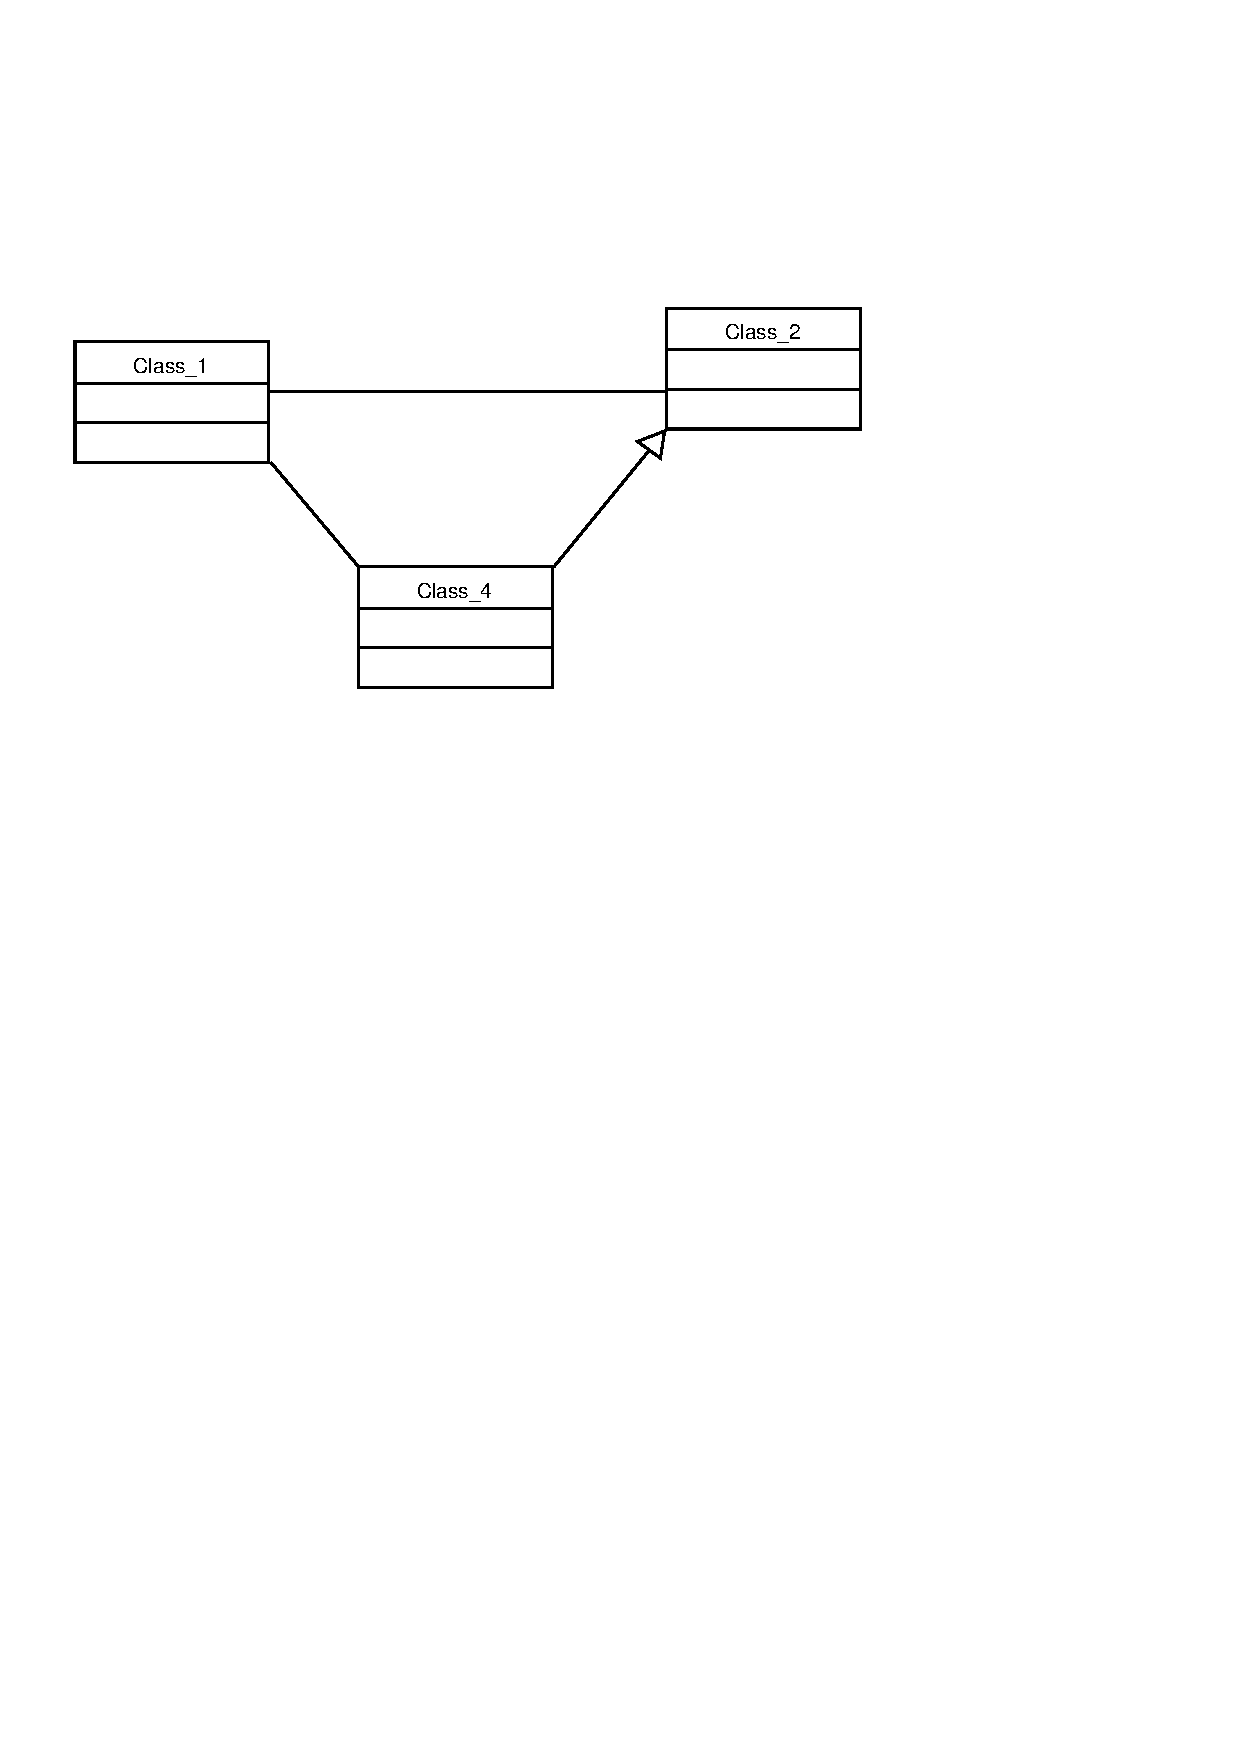
\includegraphics[width=12cm]{schema}
 \caption{Diagramma delle classi}
% \label{}
\end{figure}

\section{Dati all'interno della cache}

\subsection{Streams}

Le streams ricevuti dai server vengono salvate utilizzando direttamente
i pacchetti ricevuti. Questo viene fatto tenendo in considerazione
che i pacchetti RTP contengono nella loro instestazione un \emph{timestamp}
che identifica univocamente la posizione temporale del pacchetto all'interno
della stream audio o video.

Inoltre, considerato che un client potrebbe richiedere che lo streaming
di una risorsa cominci non dall'inizio ma da un certo istante, � possibile
che venga salvato nella cache un segmento parziale della stream originaria.
Una possibile soluzione � quella di salvare in file separati i vari
segmenti di stream dovuti a richieste {}``parziali'' dei client,
e di lasciare al Cache manager il compito di ricostruire la stream
intera a partire dai vari segmenti.

Un ulteriore passo potrebbe essere quello di mantenere una \emph{bitmap}
in memoria, associata ad un oggetto Stream (e non ad un segmento)
che indichi quali pacchetti sono effettivamente memorizzati in cache
e quali no. Questo approccio porterebbe anche il vantaggio di poter
utilizzare i contenuti presenti nella cache quando possibile, e di
richiedere lo streaming al server alla fine del segmento parziale
che si stava utilizzando.


\subsection{Ricerca}

I dati relativi alle varie stream contenute nella cache vengono
mantenuti all'interno di una lista concatenata che conterr� tutti i
riferementi necessari. Tra di essi, vi sar� anche un'ulteriore lista,
contenente i riferimenti a tutti i segmenti associati allo stream in
questione. 

La lista utilizza chiave numerica per minimizzare i tempi di ricerca
all'interno di essa. Questa chiave viene ricavata eseguendo un
checksum sull'URL della risorsa associata. 


\subsection{Rimozione di elementi dalla cache}

� normale che per una cache venga fissata una dimensione massima che
limiti la quantit� di dati che possono venire memorizzati. Questo
implica la presenza di un sistema che decida, qualora si presenti
questa situazione, quali streams debbano essere cancellate dalla cache.

Lo {}``scopo finale'' � quello di minimizzare la banda utilizzata
quindi identificare le streams \emph{meno importanti}, ed estrarle
dalla cache. Ci sono diverse approcci a questo problema e diversi
algoritmi per risolverlo. Uno dei pi� semplici � il cosiddetto LRU
(Last Recently Used), che si basa sul concetto che una risorsa che
non riceve accessi da molto tempo {}``probabilmente'' non ne ricever�
nell'immediato futuro.

Per implementare questo algoritmo si pu� utilizzare come riferimento
la lista contenente i dati relativi agli streams in cache. Se si mantiene
ordinata questa lista in base agli accessi, risulter� molto semplice
scegliere l'elemento da estrarre. Infatti, se ogni nuovo elemento
viene aggiunto inizialmente in cima alla lista, e riportato in quella
posizione ogni qualvolta venga riutilizzato, la lista risulter� ordinata
in base all'istante dell'ultimo accesso. Di conseguenza, quando ci
sar� da estrarre un elemento, verr� estratto l'ultimo elemento  
della lista, che risulter� essere quello \emph{last recently used}.


\section{Streaming verso il client}

Al momento la parte pi� complicata da realizzare sembra essere quella
che deve effettivamente inviare i pacchetti al client. Questo perch�
la situazione � differente dal caso del proxy puro, nel quale si ricevono
i pacchetti e si inoltrano immediatamente gli stessi al client, lasciando
a client e server il compito di effettuare i controlli di flusso.
In questo caso il proxy si occupa solamente di creare un canale {}``virtuale''
di comunicazione tra client e server.

Quando invece il proxy deve utilizzare i contenuti salvati nella cache,
si deve effettivamente comportare come se fosse un server, provvedendo
quindi ad effettuare un controllo di flusso sulle stream che invia.

Nell'implementazione del proxy di Real Networks � presente un metodo
che viene invocato quando si verifica l'evento di ricezione di un
pacchetto UDP; in questo metodo l'unica operazione compiuta � quella
di inviare il pacchetto ricevuto al client o al server.

Quando si sta effettuando lo streaming di dati presenti in cache,
al posto di questo metodo ne deve essere eseguito uno che, invece
di fare da forwarder, analizzi i pacchetti, specialmente quelli RTCP,
in modo da intercettare gli aknowledgement del client.

\section{Changelog}

Modifiche apportate al proxy originale di RealNetworks.

\begin{itemize}


\item Aggiunto il codice che in seguito alla richiesta \fx{SETUP}
  del client chiede al sistema di cache di verificare la presenza
  della risorsa ed attiva il meccanismo di caching.
  
\item Aggiunte le classi Cache, CacheItems e CacheSegment con le
  seguenti finalit�:

  \begin{itemize}

  \item Cache: \\
    Gestore del sistema di caching. Viene creata un'istanza
    di questa classe relativa all'applicazione, dalla quale sar� poi
    possibile accedere a tutte le sue funzioni attraverso riferimenti.
  
  \item CacheItems:\\
    Gestore della lista di oggetti presenti nella cache. Questa classe
    comprende quindi metodi per aggiungere elementi alla cache e
    controllarne l'eventuale presenza al momento di una richiesta da
    parte di un client.

  \item CacheSegment:\\
    Questa classe gestisce il salvataggio su disco dei pacchetti che
    transitano nel proxy. Viene creata una nuova istanza per ogni
    stream richiesta dal client non presente in cache. � quindi
    previsto che ci possano essere pi� CacheSegment per una sola
    richiesta RTSP, in relazione al fatto che per lo streaming di un
    filmato vengono inviate 2 stream, una audio ed una video.\\
    Viene quindi creata una lista di CacheSegment che referenzia
    questi oggetti.

  \end{itemize}    

\item Aggiunte opzioni da linea di comando per abilitare il sistema di cache

\item Modificato il sistema di compilazione utilizzando autoconf/automake per 
  aver maggiore flessibilit�.
  
\end{itemize}

\end{document}
